
\section{Experimentálne určenie hustoty stavov elektrónov v kovoch}
V tejto kapitole popíšeme, ako experimentálne merať hustotu stavov v disorderovanom kove. Využijeme pri tom efekt tunelovania cez 
potenciálovú bariéru, ktorú bude predstavovať izolant medzi dvoma kovmi. Na ľavo máme veľmi čistý kov so známou hustotou stavov.
Na pravo máme skúmaný kov z neznámou hustotou stavov. Izolant medzi kovmi tvorí potenciálovú bariéru, cez ktorú musia elektróny pretunelovať. 
\subsection{Tunelovanie a Fermiho zlaté pravidlo}
Tunelovanie cez potenciálnu bariéru $V(x)$ má hamiltonián:
\begin{equation}
 \label{eq:exp_barrier}
 \hat{H}=\frac{\hbar^2 \laplace }{2m}+V(x) \text{,}
\end{equation} 

kde:
\begin{equation}
 \label{eq:exp_potential_barrier}
 V(x)=
 \begin{cases}
    V_0,& \text{pre } 0<x<b\\
    0,              & \text{inak}
\end{cases}\text{,}
\end{equation} 
kde $b$ je šírka bariéry. Tento problém sa tradične rieši nájdením vlnovej funkcie v troch oblastiach potenciálu, a následným zlepením
riešenia pomocou spojitosti vlnovej funkcie a jej derivácie.

Na celú vec sa však dá pozrieť aj inak, a to určením vlnových funkcii $\psi_l$ a $\psi_r$ pre nekonečne širokú bariéru zľava $V_l(x)$ a  
sprava $V_r(x)$, teda:
\begin{equation}
 \label{eq:exp_potential_left}
 V_l(x)=
 \begin{cases}
    V_0,& \text{pre } 0<x\\
    0,              & \text{inak}
\end{cases}\text{,}
\end{equation} 
a podobne sprava
\begin{equation}
 \label{eq:exp_potential_right}
 V_r(x)=
 \begin{cases}
    V_0,& \text{pre } b>x\\
    0,              & \text{inak}
\end{cases}\text{.}
\end{equation} 
Pre oba potenciály možno určiť vlnové funkcie   $\psi_l(x)$ a $\psi_r(x)$.  Treba poznamenať, že stavy $\psi_r(x)$ a $\psi_l(x)$ 
môžu mať rôzne kvantové čísla $l$ a $r$.

Funkcia $\psi_l(x)$ je očividne dobrou aproximáciou stavu častice na ľavo od bariéry $V(x)$. Nieje však stacionárnym stavom príslušného hamiltoniánu \eqref{eq:exp_barrier}, preto musíme riešiť časovú SchR:
\begin{equation}
 \label{eq:exp_time_schr}
 i\hbar \frac{d}{dt}\psi(x,t)=\hat{H} \psi(x,t)\text{.}
\end{equation} 
Časticu je v čase $t=0$ na ľavo od bariéry teda v stave $\psi_l(x)$, čo nám dáva počiatočnú podmienku:
\begin{equation}
 \label{eq:exp_init_cond} 
 \psi(x,0)=\psi_l(x)\text{.}
\end{equation} 
Vieme, že častica má nenulovú pravdepodobnosť pretunelovať doprava. Zároveň považujeme prechod za elastický, teda budeme riešenie 
\eqref{eq:exp_time_schr} hľadať v tvare:
\begin{equation}
 \label{eq:exp_time_schr_solution}
 \psi(x,t)=c_l(t)\psi_l(x)e^{-\frac{iE_l t}{\hbar}}+\sum_{\forall r} c_r(t)\psi_l(x)e^{-\frac{iE_r t}{\hbar}}\text{,}
\end{equation} 
kde s počiatočných podmienok \eqref{eq:exp_init_cond} dostávame:
\begin{equation}
 \label{eq:exp_time_schr_coeficients} 
c_l(0)=1 , c_r(0)=0 \text{.}
 \end{equation} 
 
Pre slabo preniknuteľnú bariéru vieme koeficienty aproximovať ako:
 \begin{equation}
 \label{eq:exp_time_schr_coeficients_approx} 
c_l(t)\doteq1,c_l'(t)\doteq1 , c_r(t)\doteq0 \text{.}
 \end{equation} 
 
Dosadením \eqref{eq:exp_time_schr_solution}  do \eqref{eq:exp_time_schr} a použitím \eqref{eq:exp_time_schr_coeficients_approx} 
a následnými úpravami dostaneme pravdepodobnosť prechodu zo stavu naľavo $l$ do stavu napravo $r$ za jednotku času ako:
\begin{equation}
 \label{eq:exp_golden_rule}
 w_{r\to l}=\frac{2\pi}{\hbar} \bra{\psi_l}H-E_l\ket{\psi_r}\delta(E_l-E_r)\text{.}
\end{equation} 
Dostali sme vzťah podobný Fermiho Zlatému pravidlu, známy ako Bardinovo zn
\subsection{I-V charakteristika tunelového spoja}
Vypočítali sme pravdepodobnosť tunelovania za jednotku času, presnejšie pravdepodobnosť prechodu z konkrétneho stavu naľavo, do konkrétneho
stavu napravo. Z toho vieme vypočítať I-V charakteristiku, čo je dôležité preto, lebo sme ju schopný merať.

Sústavu kov-izolant-kov zapojíme na zdroj napätia $U$. Napätie nám spôsobí zmenu dna energetického pásu na pravej strane o $\Delta E_c$.
Potenciálová bariéra už nebude ako v prípade \eqref{eq:exp_potential_barrier} ale bude mať kôli zdroju napätia tvar lineárnej funkcie.
(pozri obrázok).
\begin{figure}[H]
\centering
 \includegraphics[scale=0.3]{grafy/Barier.pdf}
 \caption{Asymetrická potenciálová bariéra a náčrt stavu $\psi_l$ s energiou $E_l$ naľavo
 od bariéry a stavu $\psi_r$ a $\psi_l$ napravo od bariéry. O týchto stavoch
 vieme, že nie sú vlastné stavy hamiltoniánu. V praxi sa bežne postupuje formálne tak, 
 že $\psi_l$ a $\psi_r$ sa  nerátajú, a maticový element ${\bra{\psi_r}H-E_l\ket{\psi_l}}$
 je parameter teórie.}
\end{figure}


Obsadzovacie čísla jednotlivých elektrónových stavov budú na ľavo dané Fermi-Diracovým rozdelením:
\begin{equation}
 \label{eq:exp_fermidirac_left}
 f_l(k_l)=\frac{1}{e^{\frac{E_{k_l}-\mu_l}{k_bT}}+1}\text{,}
\end{equation} 

podobne pre stavy na pravo:

\begin{equation}
 \label{eq:exp_fermidirac_right}
 f_r(k_r)=\frac{1}{e^{\frac{E_{k_r}-\mu_r}{k_bT}}+1}\text{.}
\end{equation} 

Pri odvodení zlatého pravidla \eqref{eq:exp_golden_rule} sme nikde explicitne nevyužili, že bariéra má tvar
\eqref{eq:exp_potential_barrier}, preto ho zrejme môžme použiť pre náš potenciál.

Počet elektrónov, ktoré za jednotku času prejdú zľava do prava je 
\begin{equation}
 \label{eq:exp_ltr}
 \Gamma^+(\Delta E)=2\sum_{\forall k_l}\sum_{\forall k_l} w_{k_l\to k_r} f_l(k_l)[1-f_r(k_r)]\text{,}
\end{equation} 
výraz $[1-f_r(k_r)]$ je pravdepodobnosť že stav je voľný, čo vyžaduje Pauliho princíp. Podobný výraz dostaneme pre prechod sprava do ľava.

\begin{equation}
 \label{eq:exp_rtl}
 \Gamma^-(\Delta E)=2\sum_{\forall k_l}\sum_{\forall k_l} w_{k_r\to k_l} f_r(k_r)[1-f_l(k_l)]\text{.}
\end{equation} 
Zo vzťahov \eqref{eq:exp_ltr} a \eqref{eq:exp_rtl} potom dostaneme:
\begin{equation}
 \label{eq:exp_current}
 I=e[\Gamma^+(\Delta E)-\Gamma^-(\Delta E)] \text{.}
\end{equation} 

Dosadením \eqref{eq:exp_ltr} a \eqref{eq:exp_rtl} do \eqref{eq:exp_current} a prejdení od sumy k integrálu dostaneme:
\begin{equation}
\label{eq:exp_current_2}
I=e\int d\vk_r \int \vk_l w_{k_l\to k_r} f_l(k_l)[1-f_r(k_r)] -  w_{k_r\to k_l} f_r(k_r)[1-f_l(k_l)]\text{.}
\end{equation} 
Vo $w_{k_l\to k_r}$ máme $\delta(E_l-E_r)$ prejdeme teda do energetických súradníc a jednu z nich využijeme,
dostaneme:
\begin{equation}
 \label{eq:exp_current_3}
 I=e\frac{4\pi|t^2|}{\hbar}[\int_{E_{cl}}^{\infty}dE_lN_e{E_l}N_r{E_l}(f_l(E_l)-f_r(E_l)) ]\text{,}
\end{equation} 
kde $N_l(E_l)$ a $N_l(E_l)$ sú hustoty stavov naľavo a napravo od bariéry a $t$ je transmisný koeficient. Celý problém riešime v limite nízkych teplôt,
kde nám Fermi-Diracove rozdelenia prejdú na $\Theta$-funkcie, teda výraz \eqref{eq:exp_current_3} prejde na:
\begin{equation}
 \label{eq:exp_current_lt}
 I=e\frac{4\pi|t^2|}{\hbar} [\int_{E_{cl}}^{\mu_l} dE_l 
 N_r(E_l)
 N_l(E_l)
 -\int_{E_{cl}}^{\mu_r}
 dE_l 
 N_r(E_l) N_l(E_l)] \text{,}
\end{equation} 
keďže chemický potenciál naľavo a napravo sa líši o $\delta E=-Ue$, kde $U$ je napätie zdroja dostávame finálny vzťah pre prúd.
\begin{equation}
 \label{eq:exp_current_lt_final} 
  I=e\frac{4\pi|t^2|}{\hbar} [\int_{\mu_r}^{\mu_r-Ue} dE_l N_r(E_l) N_l(E_l)\text{.}
\end{equation} 

\subsection{Určenie hustoty stavov}
Odvodili sme vzťah medzi prúdom a napätím (I-V charakteristiku) pre tunelový spoj dvoch kovov. Vidíme, že napätie závisí 
od hustoty stavov naľavo a napravo. Kov naľavo je čistý, bez disorderu, preto poznáme jeho hustotu stavov. Preto vieme 
vyjadriť hustotu stavov pre neznámy kov napravo. 

Chemický potenciál $\mu_r$ je rádovo desiatky eV. Rozdiel energií $\Delta E$ je rádovo stovky meV. Hustota stavov $N_l(E_l)$ 
sa teda v okolí $\mu_r$ dá aproximovať konštantou $N_l(\mu_l)$ a vyňať pred integrál. 



\begin{figure}[H]
\begin{center}
 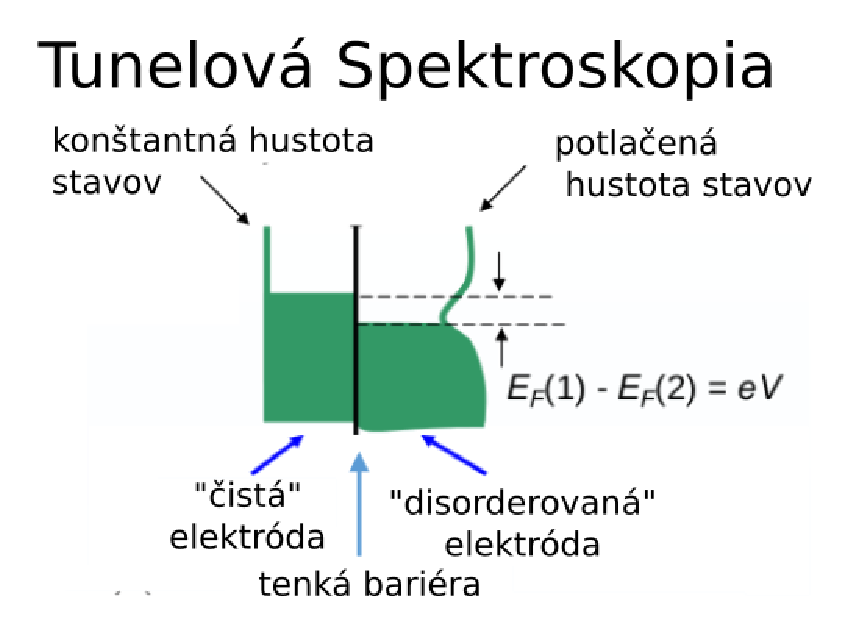
\includegraphics[scale=0.7]{grafy/DOS-sk.eps}
 \end{center}
 \caption{Meranie hustoty stavov tunelovou spektroskopiou. V experimente máme "čistý" a "disorderovaný" kov, 
 oddelené sú tenkou vrstvou izolantu, ktorý tvorí potenciálovú bariéru. Meraná veličina je diferenciálna
 vodivosť $\frac{dI(U)}{dU}=G(U)$. Vzťah medzi diferenciálnou vodivosťou a hustotou stavov je 
 $\frac{\rho(\epsilon)}{\rho_0(0)}=\frac{G(U)}{G_0(U)}$; kde $G_0$ je diferenciálna vodivosť v prípade, 
 že na oboch stranách máme "čistý" kov.}
 \label{fig:exp_dos_meranie}
\end{figure} 
Hľadanú hustotu stavov máme teraz pod integrálom. Preto je vhodné určiť difernciálnu vodivosť:
\begin{equation}
 \label{eq:exp_current_der}
  \frac{dI}{dU}=e\frac{4\pi|t^2|}{\hbar} N_l(\mu_l) N_r(\mu_r-Ue)
\end{equation} 
Deriváciu prúdu podľa napätia určíme z I-V charakteristiky. Hustotu stavov vieme vyjadriť ako funkciu merateľných veličín.
\begin{equation}
 \label{eq:exp_dos}
 N_r(\mu_r-Ue)= \frac{\frac{dI}{dU}(U)}{e\frac{4\pi|t^2|}{\hbar}}=\alpha \frac{dI}{dU}(U)
\end{equation} 
kde konštantu $\alpha$ môžme určiť fitovaním.

Pri odvodení vzťahu pre deriváciu prúdu \eqref{eq:exp_current_der} sme predpokladali, že od napätia závisí iba hustota stavov.
Vo všeobecnosti to však nieje pravda, pretože aj tunelový koeficient $t(U)$ je funkciou napätia. V našom prípade lineárne klesajúcej bariéry
tým získa meraná hustota stavov \eqref{eq:exp_dos} parabolické pozadie. 
\begin{figure}[H]
\begin{center}
 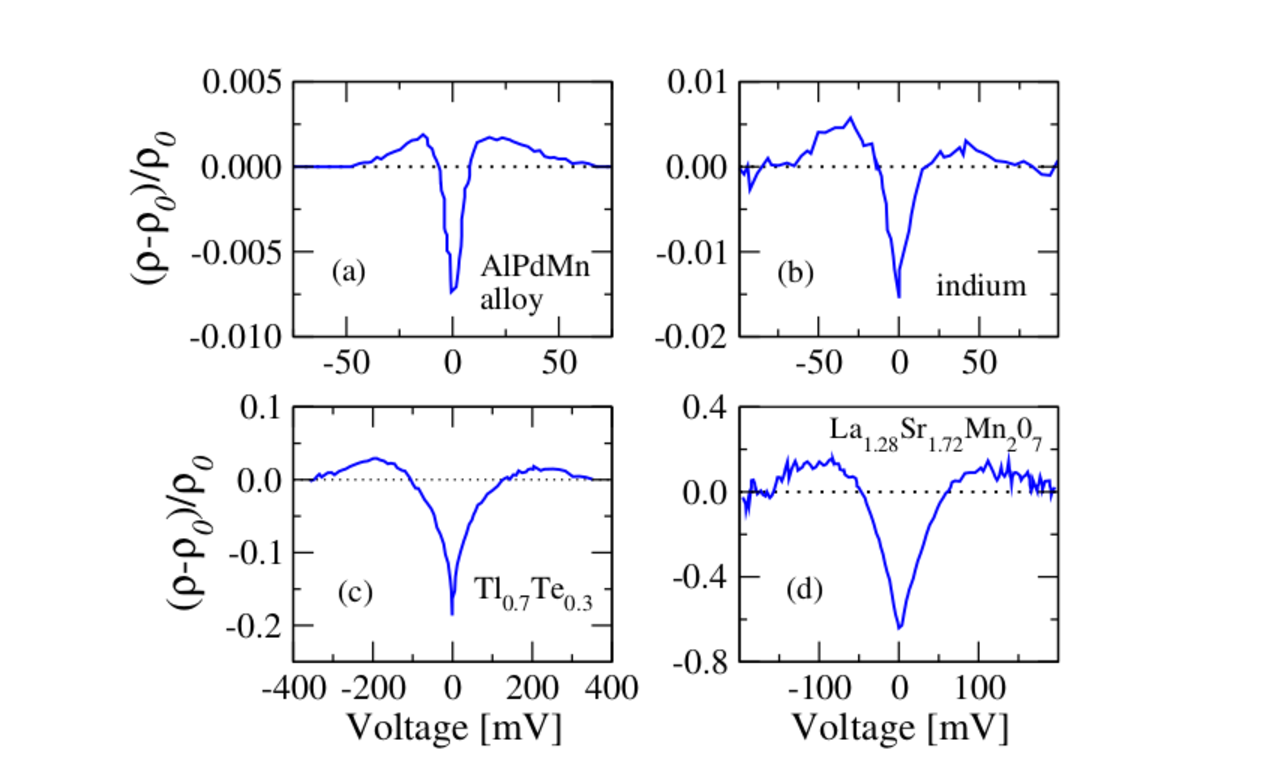
\includegraphics[scale=0.7]{grafy/B2}
 \end{center}
 \caption{Výsledky merania hustoty stavov tunelovou spektroskopiou pre rôzne kovy a zliatiny. Vo výsledných grafoch 
 môžme vidieť pokles hustoty stavov v okolí Fermiho energie}
 \label{fig:exp_results} 
\end{figure}

